\chapter{Towards the Systematization of Glyph Design}

\label{chap:strategies}
The design of glyphs is largely an ad-hoc process, mainly informed by the tasks a user wishes to perform and relying of the craftsmanship of a designer to bring together domain knowledge and intuition into an aesthetically pleasing yet functional end product.
Although this may work in simple cases, it may also result in: 
\begin{enumerate}
\item incorrect mapping of data types to visual channels; 
\item visual channels overloading by attaching too many data types (\eg too many colours); 
\item information obfuscation by overcrowding at a working resolution; and 
\item indecipherable glyphs to the intended target audience. 
\end{enumerate}

Recent work by Colin Ware \cite{ware13} has gone some way to providing designers with insights about the workings of the visual system. 
Such work brings together knowledge of visual information processing investigated by psychologists and neuroscientists, familiarizes designers with essential mechanisms they can tap into to create principled, innovative and effective visualizations.\\

%
%\begin{figure}[ht!]
%\centering
%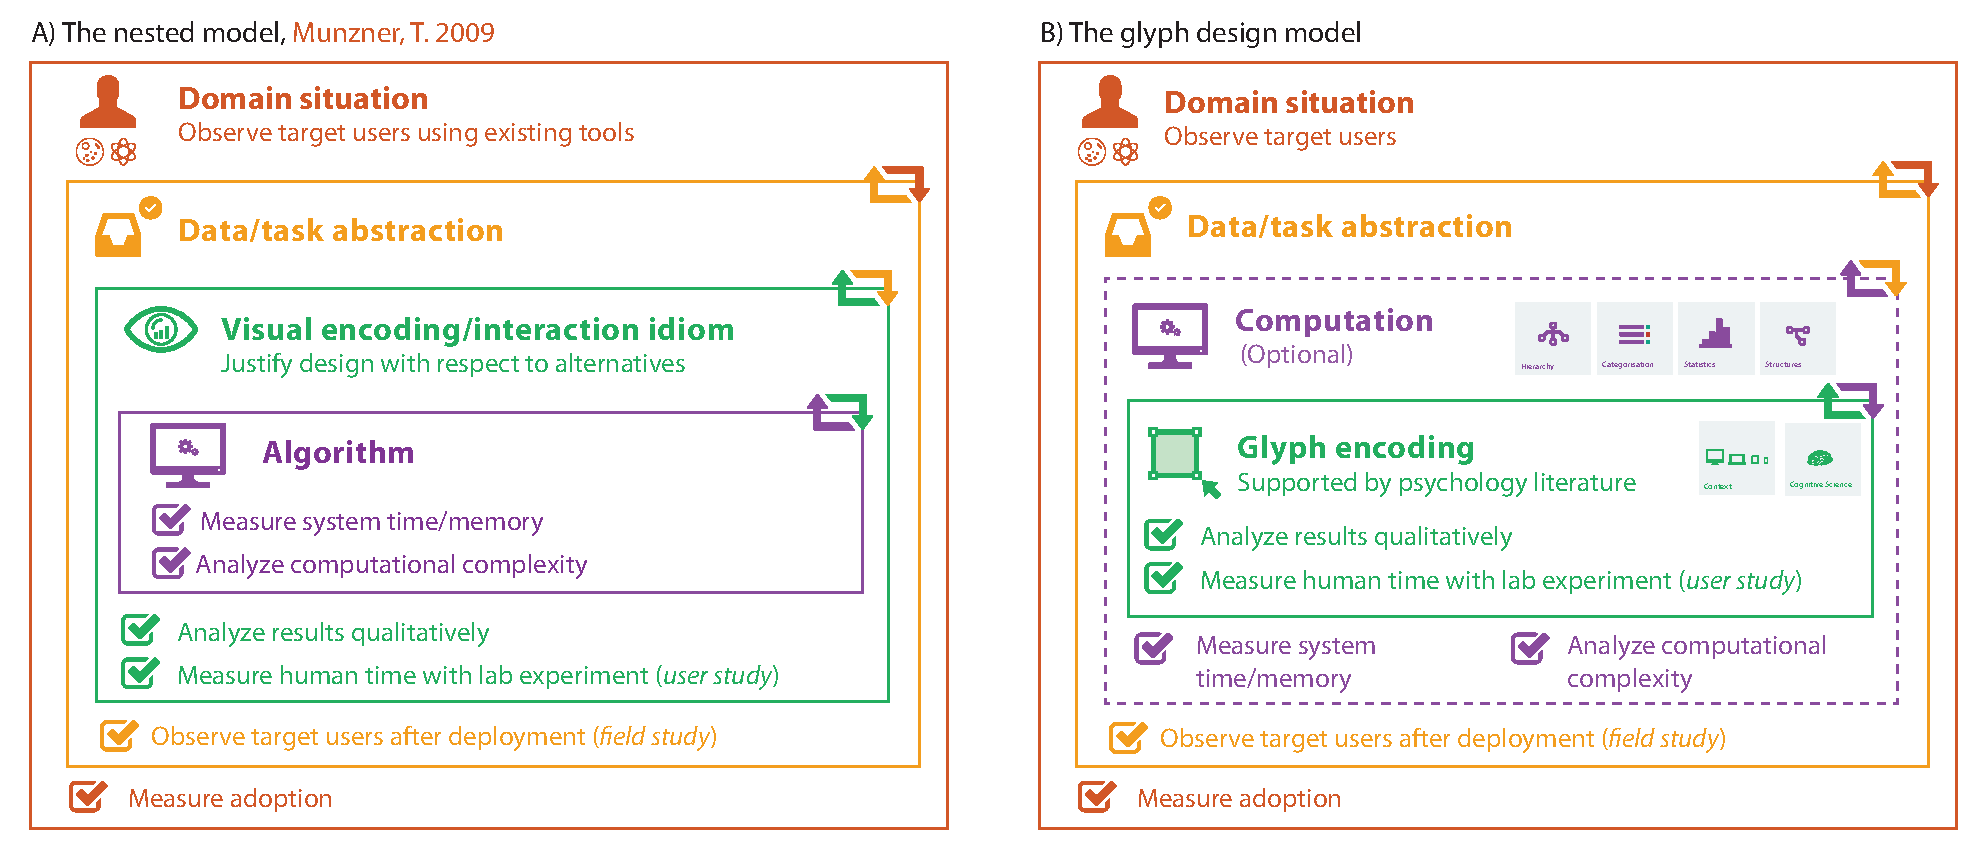
\includegraphics[width=\textwidth]{images/ch3/model}
%\caption{A) An overview of the ``nested model'' presented by Munzner \etal \cite{munzner2009nested}. B) A ``glyph design model'' inspired by the ``nested model''.}
%\label{fig:systematisation-models}
%\end{figure}

\begin{chapquote}{V. Gordon Childe}{``The aim of science is surely to amass and systematize knowledge''}
\end{chapquote}

\begin{figure}[h!]
\centering
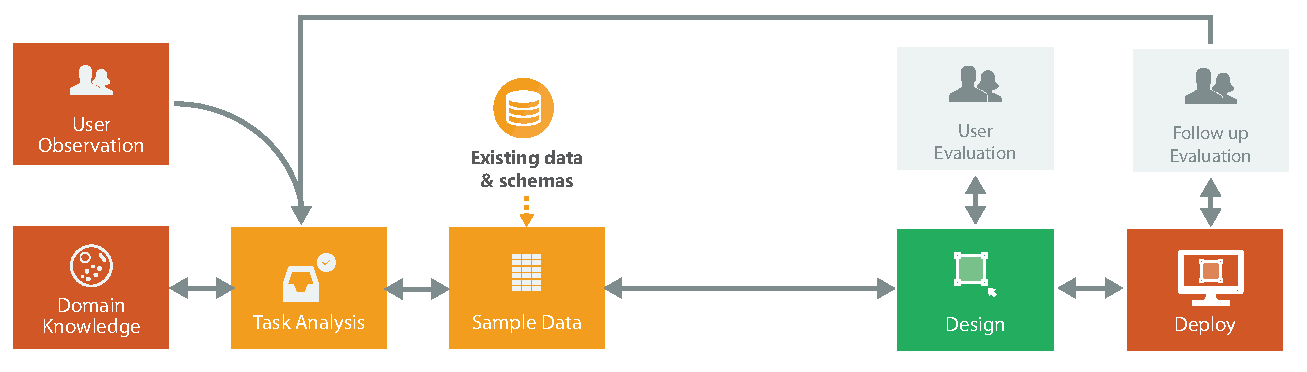
\includegraphics[width=\textwidth]{images/ch3/model_horizontal_simple}
\caption{A typical glyph design process modelled upon the ``nested model'' by Munzner \cite{munzner2009nested} : the iterative cycle of domain expert input, designer creative interpretation, appraisal and interaction in the glyph production process.}
\label{fig:simple_process}
\end{figure}


Figure \ref{fig:simple_process} illustrates the standard process behind  glyph creation, mapped to the components of the frequently followed ``nested model'' for visualization design by Munzner \cite{munzner2009nested}.
This model has the following components at its core:

\begin{itemize}
\item \textbf{User Observation:} quite frequently, domain experts play an essential part in the design process, feeding into:
\begin{enumerate}
	\item \emph{task definition:} by means of interviews and day to day observations of current working practices;
	\item \emph{design process:} by taking into account a user is willing to learn, willing to remember or able to remember. This ultimately determines the number of variables available to encoding and how those should be encoded. If the glyph recall time available to the user is limited or restricted, a stronger reliance on metaphor, for instance, could be sought to support performance.
	\item \emph{evaluation process:} to assess glyph design fitness for purpose and match user expectations against the initial problem the glyph was meant for.
\end{enumerate}
\item \textbf{Domain Knowledge} is central to in any visualization as it drives the unambiguous definition of the problem at hand, an essential first step to devising  better visualization solutions.
Furthermore, domain knowledge carries additional importance in glyph-based visualization  as it affords for more competent and effective metaphors to be developed in support of glyph learnability and memorability;

\item \textbf{Task Analysis} (or data/task abstraction in the ``nested model'') provides an indication of the nature of visual explorations a user would like to make.
These tasks form the basis of data prioritization, the process of associating key variables to the strongest known visual cues. For example, if a major task performed by a user was finding users of a particular age, making the age information more visually available is important;

\item \textbf{Sample Data} inform on the data values (and ranges) to be encoded by the glyphs.
%These values can be processed by algorithms (see the \emph{computation} section) to find the most common values, the rarest values, and so forth depending on the visualization requirements.
The \emph{Data Representation Schema} can provide additional information about the format of the sample data and the types of values  (\eg, categorical or quantitative) each field contains.
This in turn can be used in the design phase, where design guidelines, discussed below, can be applied to ensure that most suited visual channels are matched to relevant data values;

\item \textbf{Design} involves the selection of appropriate visual channels to represent each data variable to be encoded, followed by the arrangement of those visual channels in 2D or 3D space;
%	\begin{itemize}
%		\item \textbf{Context}, which defines the environment (\eg devices available) in which the glyphs are being used. \emph{Users} and their \emph{tasks} will have different requirements based on the environment being worked in.
%		If a set of glyphs are being presented on a power wall in a situation control room in one scenario versus a desktop in another, the glyphs may need to be designed differently. 
%		There would be little point in having thin lines with a high spatial frequency on a screen too far away for users to view. 
%		It would also be ill advised to use particular colours maps when 3D is a requirement since lighting effects such as shadowing can change how particular hues are rendered.
%		\item \textbf{Cognitive Science}:
%			\begin{itemize}
%				\item \emph{users} and their ability and/or willingness to learn and remember is an important consideration in any glyph design. 
%				A user with little time to learn a new visual language will not want very complex glyphs; and
%				For instance a cardiovascular surgeon using glyphs to show properties of the heart during surgery may not have the time to remember how five or six variables are mapped to retinal variable without having to consult a lookup chart;  
%				\item \emph{tasks} are important to cognitive science since variables that are important in achieving particular tasks can be emphasized more than variables of a lesser importance.
%				``High value'' information, important for completion of priority tasks should be visualized using powerful visual channels such as position or colour for example;
%				``Low value'' information that is more often utilized when diving in to more detailed views should be encoded using less powerful visual channels in less prominent positions within the glyph;
%				\item \emph{data schemas} provide an overview of the data types to be visualized including whether the values are quantitative or qualitative.
%				As shown in Chapter \ref{chap:related_work}, some visual channels are better suited to data type than others.
%				For example colour hue is not well suited to quantitative variables but position is. Conversely, colour hue works well as a means for representing categorical (qualitative) information;
%				\item \emph{data values} are useful at the design phase as a further way of determining a suitable mapping from the data value to its retinal variable.
%				For instance, for categorical information, it is estimated that between eight and twelve colours can be observed distinctly \cite{ware13}. If there are more categories it may be better to consider an alternative mapping; and
%				\item \emph{computational results} can provide the hierarchy, clusters, structures or statistics that may help in determining the most important features of the data. 
%				This in turn may be used to support the composition of the overall glyph.
%			\end{itemize}
%	\end{itemize}

\item \textbf{Evaluation} to ascertain that the design produced meets expectations. 
This can be validated by reviewing the tasks defined earlier with users to determine if the glyphs serve their purpose. 
In case glyphs are providing an alternative to an existing visualization solution, superiority studies in the form of benchmarks on user accuracy and task speed can be carried out for comparison purposes.
In the event of the design prototype failing to surpass the alternative, further iterations may be performed to bring performance in line with target parameters. 
Once the design is approved, the glyphs can be deployed in the day to day working environment of the domain experts.
Follow up studies can be conducted, possibly leading to refinements and improvements over initial versions.
\end{itemize}

Although this model represents common visualization design practices, it does not offer direct solutions to help define a systematic approach to glyph design.
Much of the details are left up to individual designers to negotiate with domain experts.
Such visualization design process is referred to as \emph{ad hoc} (``for this'').
Owing to the need for domain specific metaphors, an \emph{ad omnia} (``for everything'') design process is unlikely to exist.
However, by incorporating principled design guidelines, a more objective decision making can be sought.
Furthermore, the addition of computational techniques bring new ways to optimize glyph design: amongst others, exploiting the statistical information and properties associated with any data set.

\begin{figure}[h!]
\centering
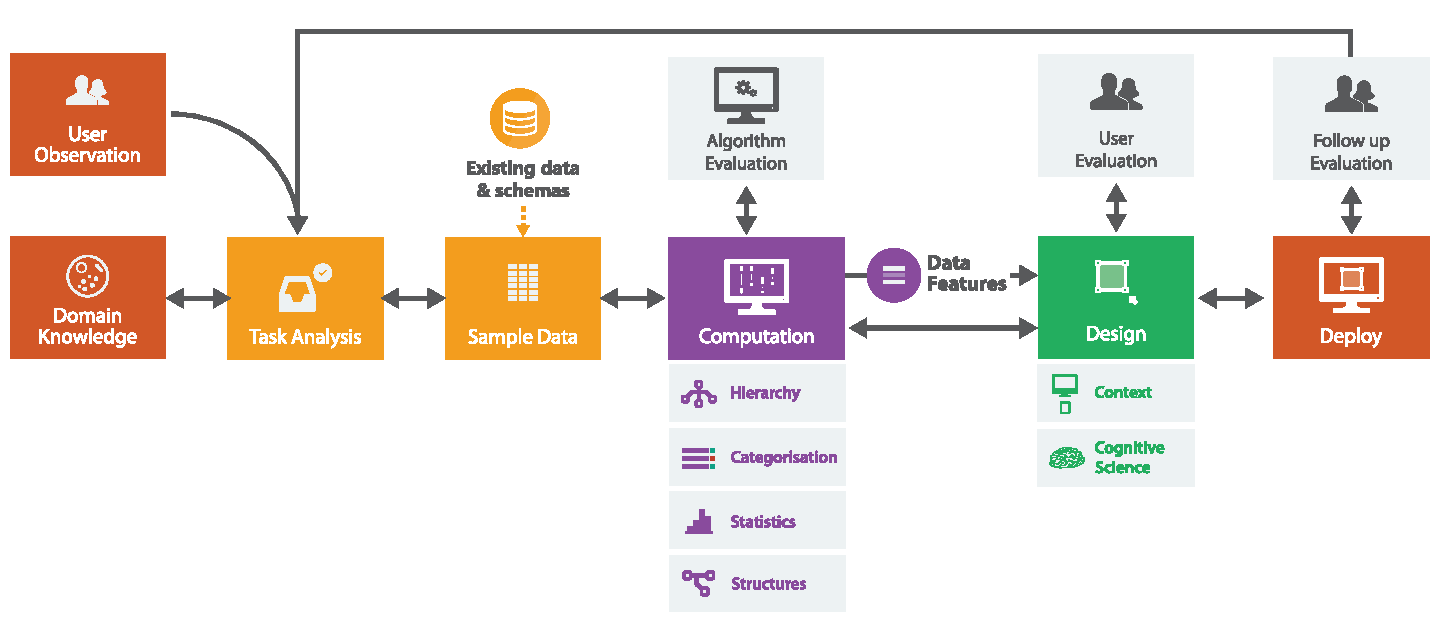
\includegraphics[width=\textwidth]{images/ch3/model_horizontal_new}
\caption{A more systematic approach to glyph creation, relying on computation and using design guidelines in context, to drive the design step.}
\label{fig:new_process}
\end{figure}

This chapter proposes an approach illustrated in Figure \ref{fig:new_process}, for the systematic creation of glyphs.
Central to this methodology is the inclusion of computational techniques to the model in Figure \ref{fig:simple_process}, and a more structured approach to the selection and arrangement of visual channels in the design step.
Our additions are meant to reduce subjectivity in the design process without departing from the ``nested model'' \cite{munzner2009nested}, thus preserving the crucial function of domain-expert interaction and evaluation, which can not be downplayed.

The remainder of this chapter delves into the details of how these \emph{design} and \emph{computation} steps break down, and how, individually and collectively, they can contribute to improving glyph design.
%First we start with design guidelines and how they can be used on their own to put systematicism in to glyph design.
%Then we discuss how computation can be used to determine which data should be represented by glyphs in compression visualizations, followed by how the results of computation can be used to inform the design process directly.

\section{Design Guidelines}

\begin{figure}[h!]
\centering
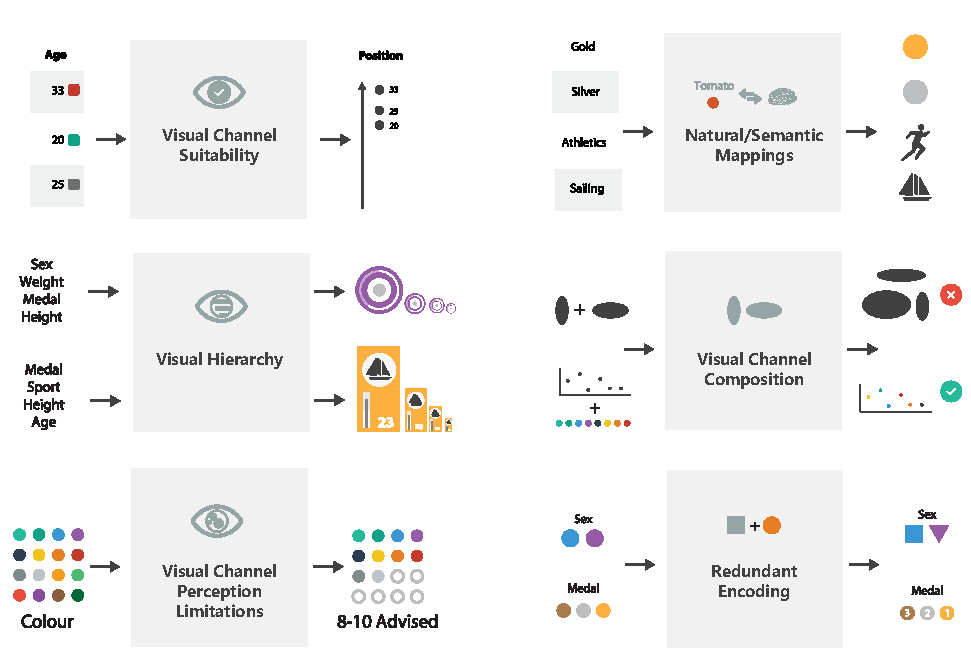
\includegraphics[width=\textwidth]{images/ch3/design_guidelines_2}
\caption{Design guidelines that can be followed to provide a more systematic approach to glyph design.}
\label{fig:strategies_design_guidelines}
\end{figure}

Ultimately, the purpose of systemizing a technique is to remove the level of randomness in a given process.
In the field of glyph design, it is our conviction that the levels of randomness can be better controlled by integrating emerging knowledge about how the visual system works.
As stated in earlier, it is unlikely that glyph design will ever become a  fully automated process, owing to the specifics of a given field. Yet fundamental principles can be drawn, building on the work presented in chapter \ref{chap:related_work}, resulting in glyphs being better designed.
Core to such a process are a set of guidelines that consists of:

\begin{enumerate}

\item \textbf{Retinal variable suitability} in Figure \ref{fig:strategies_design_guidelines} A advises that, within a glyph, data types  should be mapped to the most relevant visual channels (retinal variable suitability guidance). This is based on work by Stevens \cite{stevens1975}, Bertin \cite{Bertin:1983:book}, Cleveland and McGill \cite{cleveland1984graphical}, Mackinlay \cite{mackinlay1986automating}, Heer and Bostock \cite{heer2010crowdsourcing};

\item \textbf{Natural mappings} in Figure \ref{fig:strategies_design_guidelines} B suggests the use of semantically meaningful mappings of data to their natural visual counterparts where possible.
Using too many abstract colours or shapes, for example, would place too high a cognitive load on a user, who would probably, as a consequence, exhibit lower recall.
However, augmenting these colours or shape with metaphors makes the process of glyph decoding much easier, \eg, \textcolor{Red}{strawberry $\Leftrightarrow$ red}, \textcolor{Plum}{aubergine $\Leftrightarrow$ purple}, or \textcolor{Green}{money $\Leftrightarrow$ green} \cite{lin2013selecting}.
This guideline is based on Ware \cite{ware2010visual, ware13}, Borgo \etal \cite{Borgo12}, and Lin \etal \cite{lin2013selecting};

\item \textbf{Visual hierarchy} in Figure \ref{fig:strategies_design_guidelines} C applies an organization to the visual channels within a glyph given the importance of the data to some task.
This ensures that the most important classifiers of data are available even at the overview level of a visualization, due to their visual prominence (visual hierarchy and global/local processing \cite{palmer77, navon77, shor71, love99, kinchla79}, and the pop-out effect \cite{treisman88, Hsiao200293, williams67,quinlan87,ropinski11, kandel2012principles});

\item \textbf{Retinal variable composition} in Figure \ref{fig:strategies_design_guidelines} D suggests avoiding visual channels that are perceived holistically as opposed to separately\cite{attneave1950dimensions, shepard64, garner1970integrality, garner1974processing}. The integrality or separability of a pair of visual channels is not a binary split. However, it is largely agreed that width and height are the most integral, while position and colour are the most separable \cite{ware13}; 

\item \textbf{Retinal variable perceptual limitations} in Figure  \ref{fig:strategies_design_guidelines} E provides guidance to avoid overuse of a retinal variable such as colour whose perception degrades as the number of samples from each hue increases \cite{hitt1992retrofit, healey1996choosing, ware13}.
For example, four distinct colours is possible, but 16 distinct colours is difficult.
Colour maps like those provided in \emph{ColorBrewer} \cite{ColorBrewer} and \emph{Tableau} \cite{tableau_palettes} provide a good starting point for glyph designers; and

\item \textbf{Redundant encoding} in Figure \ref{fig:strategies_design_guidelines} F suggests the use of multiple encodings for one data item so as to minimize the chance of error when reading glyphs in a display \cite{ware13}.
For example, in Figure \ref{fig:strategies_design_guidelines} F, colour and shape are used to code sex.
Therefore, if the colour channel is impeded, shape can be used to distinguish between male and female glyphs.
\end{enumerate}

\section{Computational Techniques}

\begin{figure}[h!]
\centering
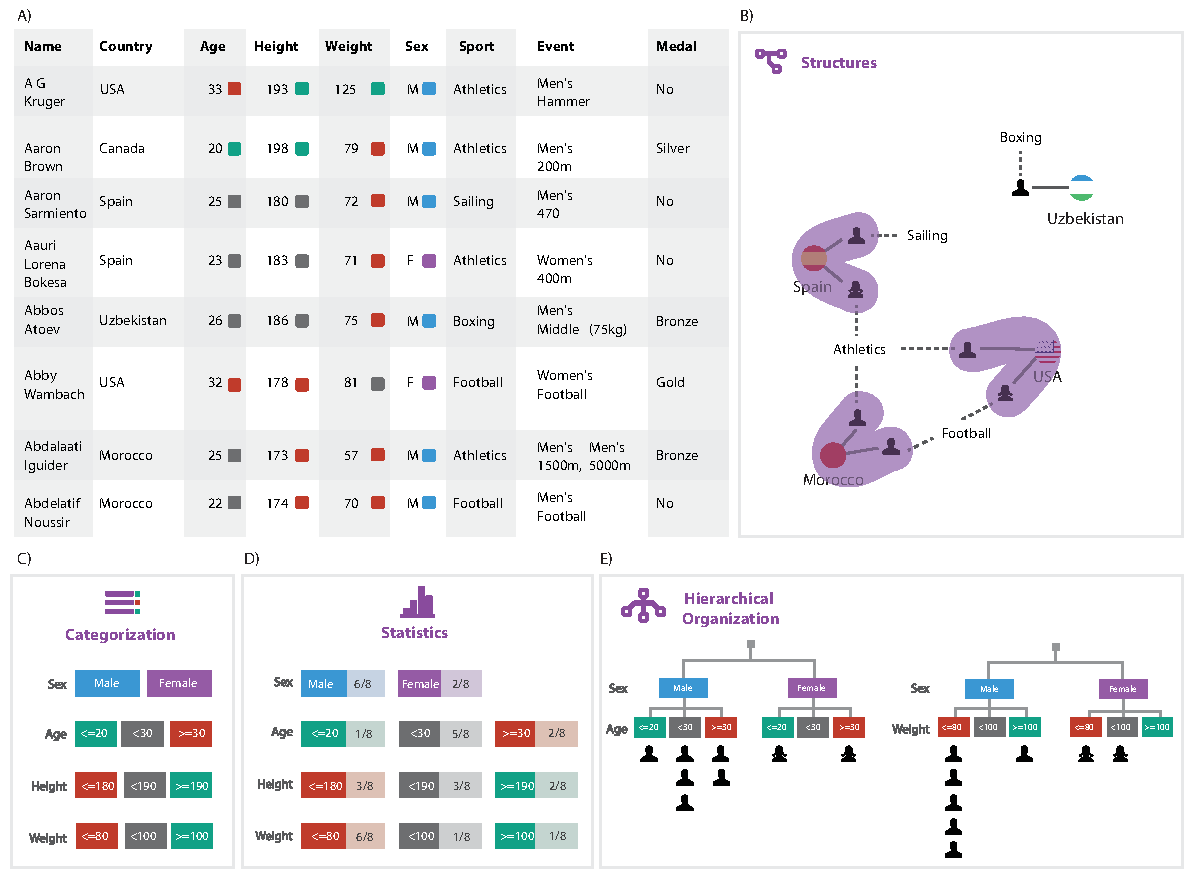
\includegraphics[width=\textwidth]{images/ch3/computation_benefits}
\caption{A) Table showing a subset of London 2012 Olympians with country, age, height, weight, sex, general sport, events, and whether they won a medal.
B) By building a graph from the data from the table in A) certain structures can be mined in the data. Common structures in graphs or motifs could be a target for aggregation when the graph is very large.
C) We can create categories from the data that can be used directly to colour code ranges of values for instance. Categories are also encoded in A).
D) Statistics can provide an indication on how balanced particular categories are, or what values are very common or very rare so that they may be highlighted or hidden depending on the user task.
E) Using categories from C) we can generate a tree/taxonomy that classifies the data in a structured way.
The choice of category will ultimately change the properties of the tree including how balanced it is (\eg, the tree on the left is more balanced than the one on the right since people are more evenly distributed at the leaf nodes).}
\label{fig:computational_benefits}
\end{figure}

Computational techniques can be deployed to provide additional information about the data that was often not obvious from the raw data.
We have identified the following four techniques, to apply either individually or combinatorially to assist the glyph design process:
\begin{enumerate}

\item \textbf{Structure identification} (Figure \ref{fig:computational_benefits} B) Generally refers to patterns in relational data, \eg, patterns in connectivity.
This information can be used in two ways: 1) for providing additional metrics for visualization through a glyph; and 2) for removing complexity in network visualizations, by eliminating common or uninteresting patterns in the data, to reveal the more salient signals.
Figure \ref{fig:structure_compress_glyph} presents a case where the goal is to detect the common elements (motifs) in a graph and substitute these motifs with less complex, glyph-based representations. 
Simple motif finding can be accomplished using an algorithm such as FANMOD \cite{wernicke06}, which identifies recurring topologies in a graph and counts their occurrence.
The most common motifs are then prioritised for substitution in a simplified graph.

\begin{figure}[h!]
\centering
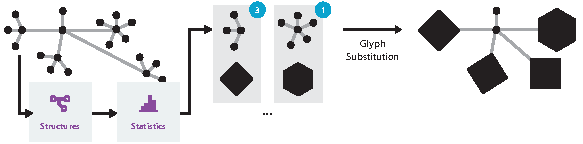
\includegraphics[width=\textwidth]{images/ch3/structure_compress_glyph}
\caption{Graph-based compression can make use of glyphs through the substitution of common structures/pattern/motifs with glyph alternatives.
This can be used to greatly reduce graph complexity as by Dunne \etal \cite{dunnemotif2012}.}
\label{fig:structure_compress_glyph}
\end{figure}

\item \textbf{Categorizations} (Figure \ref{fig:computational_benefits} C) provide a way of splitting the data based on various categorizations.
For example, in Figure \ref{fig:computational_benefits} C, there are four categories for sex, age, height and weight.
Each of these categories has a number of ``steps'', and the data is likely to be distributed differently across those different categories.
These categorization can be calculated computationally using algorithms, such as k-means \cite{macqueen1967} or hierarchical-based (\eg, \cite{Sibson01011973}) clustering.
However, these approaches are often inaccurate and computationally expensive.
Another approach is to use a more supervised approach to clustering with the aid of computation, a large representative data set, and domain experts in the loop to ensure that categorization is meaningful and not too granular.

Such categorizations, when computed, can be used to group data records based on a range of values, rather than singletons.
For example, in Figure \ref{fig:computational_benefits} C, athletes can be grouped by their age, height, or weight range.
The implications, in terms of glyph design are, that instead of representing every possible age, height, or weight, those may be represented with just three ranges showing the normal and two outlier ranges.
Going back to chapter \ref{chap:related_work}, this has implications for improving visual search. Indeed, the search space scanned for detecting a class of value has been considerably reduced , with one searching only for one of three values. Comparing between three sizes, colours, or shapes is much easier than between ten or more.

\item \textbf{Statistics} (Figure \ref{fig:computational_benefits} D) by providing insights into the distribution of the data,  statistics can feed into the categorization process for example, with possibly great benefits.
Statistical methods can also help reveal the common/rare structures, most balanced categorizations (indicative of a equiprobable chance of a record occurring in each bin).

\begin{figure}[h!]
\centering
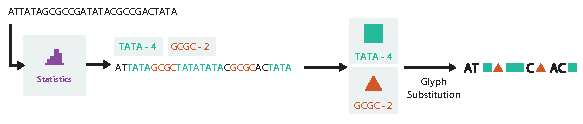
\includegraphics[width=\textwidth]{images/ch3/statistics_compression}
\caption{Text-based compression can use glyphs to replace common text with visual representations.
In this case, some common DNA motifs are replaced with coloured shapes.
Since reading text is a cognitively more demanding process than shape recognition, showing structures of interest visually can potentially speed up interpretation.
}
\label{fig:text_compress_glyph}
\end{figure}

For example, in Figure \ref{fig:text_compress_glyph} statistical processes are used to find the most common four letter sequences in a string representing a small region of DNA.
By finding the common elements and replacing them with coloured shapes, the \textcolor{green}{TATA} and \textcolor{red}{GCGC} regions can be found more easily in the DNA sequence using glyphs rather than text \cite{sperling60}.

\item \textbf{Hierarchical Organization} (Figure \ref{fig:computational_benefits} E) refers to the creation of a taxonomy, a tree representation that defines the properties of items (leaf nodes) in the tree. Examples of taxonomies in biology and visualizationa abound \cite{maguire12}, including the tree of life, in biology, that categorizes all living species by their Kingdom --> Phylum --> Class --> Order --> Family --> Genus --> Species. 
For glyph design, this hierarchical organization can be relied on the instruct how a glyph may be arranged.
Imposing an order to the design should facilitate better learnability and memorability of the resulting glyphs, as their formation follows a rule \cite{franks71}.

Figure \ref{fig:taxonomic_glyph_design} shows how one may traverse from a collection of records in a table to a taxonomic tree, then a glyph based representation of people within that tree by sex and age categories.

\begin{figure}[h!]
\centering
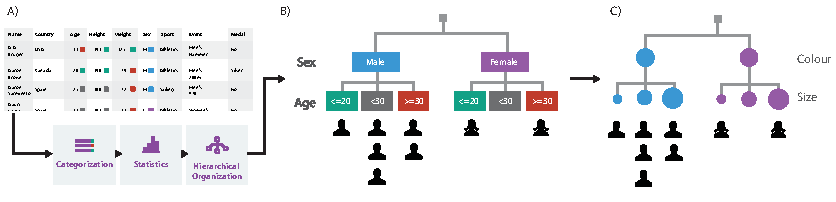
\includegraphics[width=\textwidth]{images/ch3/table_tax_glyph}
\caption{A) Starting with our table of Olympians, categorize the data, perform the statistical analysis, and generate the hierarchical organization.
B) The result of the hierarchical organization process is a taxonomic tree that represents the original data in a structured way.
C) From the hierarchical results, a glyph can be designed by assigning a retinal variable to each level in the taxonomic tree. Retinal variable use is driven by their level of popout and ability to capture attention and the level those variables occur within the taxonomic tree.}
\label{fig:taxonomic_glyph_design}
\end{figure}

\end{enumerate}


%\item \textbf{the Glyph Design Process}. Using categorization processes to find splits in the data, statistical techniques to determine how many data items are represented by such classifications, and then hierarchically arranging these classifications, a tree/taxonomy that classifies the data can be created.
%This taxonomy can be used in combination with the visual hierarchy guideline in Figure \ref{fig:strategies_design_guidelines} C to guide the glyph design process as shown in Figure \ref{fig:taxonomic_glyph_design};



%\%item \textbf{Glyph-based Compression Techniques}. Glyphs, given their ability to represent multivariate data are a perfect vector for visual compression of information.
%However, as with all compression techniques, knowing what to compress can be difficult.
%Structural pattern identification and statistical techniques can be used over a representative sample of domain data to determine the frequently occurring patterns.
%Those frequently occurring patterns can be candidates for compression. 
%Figure \ref{fig:compress_glyph} A shows an example where 






%A solid basis for such a systematic approach would be the ``nested model'' from Tamara Munzner \cite{munzner2009nested} illustrated in Figure \ref{fig:systematisation-models} A.
%This model set out with the goal of putting some structure around how visualization research is performed with respect to the requirements elicitation, visualization encoding, layout algorithm, and evaluation processes used . 
%The ``nested model'', despite its appearance is not synonymous with the \emph{waterfall model} from software engineering. 
%It is highly fluid and can involve many iterations between steps involving:
%\begin{enumerate}
%	\item observation of users in their current environment and interviewed to understand the background information for the problem;
%	\item identification of shortcomings in a users current workflow (bottlenecks), and a task list is devised with the domain experts.
%The visualization expert is often required to understand some of the principles of the domain they are working which will involve reading relevant literature and gaining a working knowledge of the domain;
%	\item devising a number of visual designs along with interactions available to the user. 
%These are refined with continuous user feedback;
%	\item devising an algorithm and other software required to create the visualization from the approved design; and
%	\item performing evaluation at all stages of the process.
%\end{enumerate}
%
%In Figure \ref{fig:systematisation-models} B we've built upon the ``nested model'' to create a model . 
%The ``nested model'' is exploratory and experimental, meaning that there are many iterations and hops back and forth between steps.
%A systematic approach would aim to remove some of the indeterminate properties of such a model. 
%The approach calls for use of computation to not only analyse the data and help in data abstraction, but also to drive the design process through the results of the computation and application of knowledge from cognitive science.
%Therefore the main difference is in the movement of computation solely as a way of implementing a design to a method that informs and supports it.
%With the addition of rules and guidelines obtained from cognitive science, we have the basis for creation of a more systematic model for glyph design.

%\section{Towards a Model for Systematization of Glyph Design}
%
%So far, we have outlined how design guidelines and computational techniques can contribute towards a systematic approach to glyph design.
%Although the aim of such an approach is to reduce subjectivity in the design process, there is always a need to interact with domain experts, since computation or following design principles alone will not result in semantically meaningful glyphs.
%Requirements elicitation, data and task abstraction, and evaluation are core to any design task.
%These facets are core to the ``nested model'' by Munzner \cite{munzner2009nested} illustrated in Figure \ref{fig:model} A which is used to guide visualization design.
%
%
%\begin{figure}[h!]
%\centering
%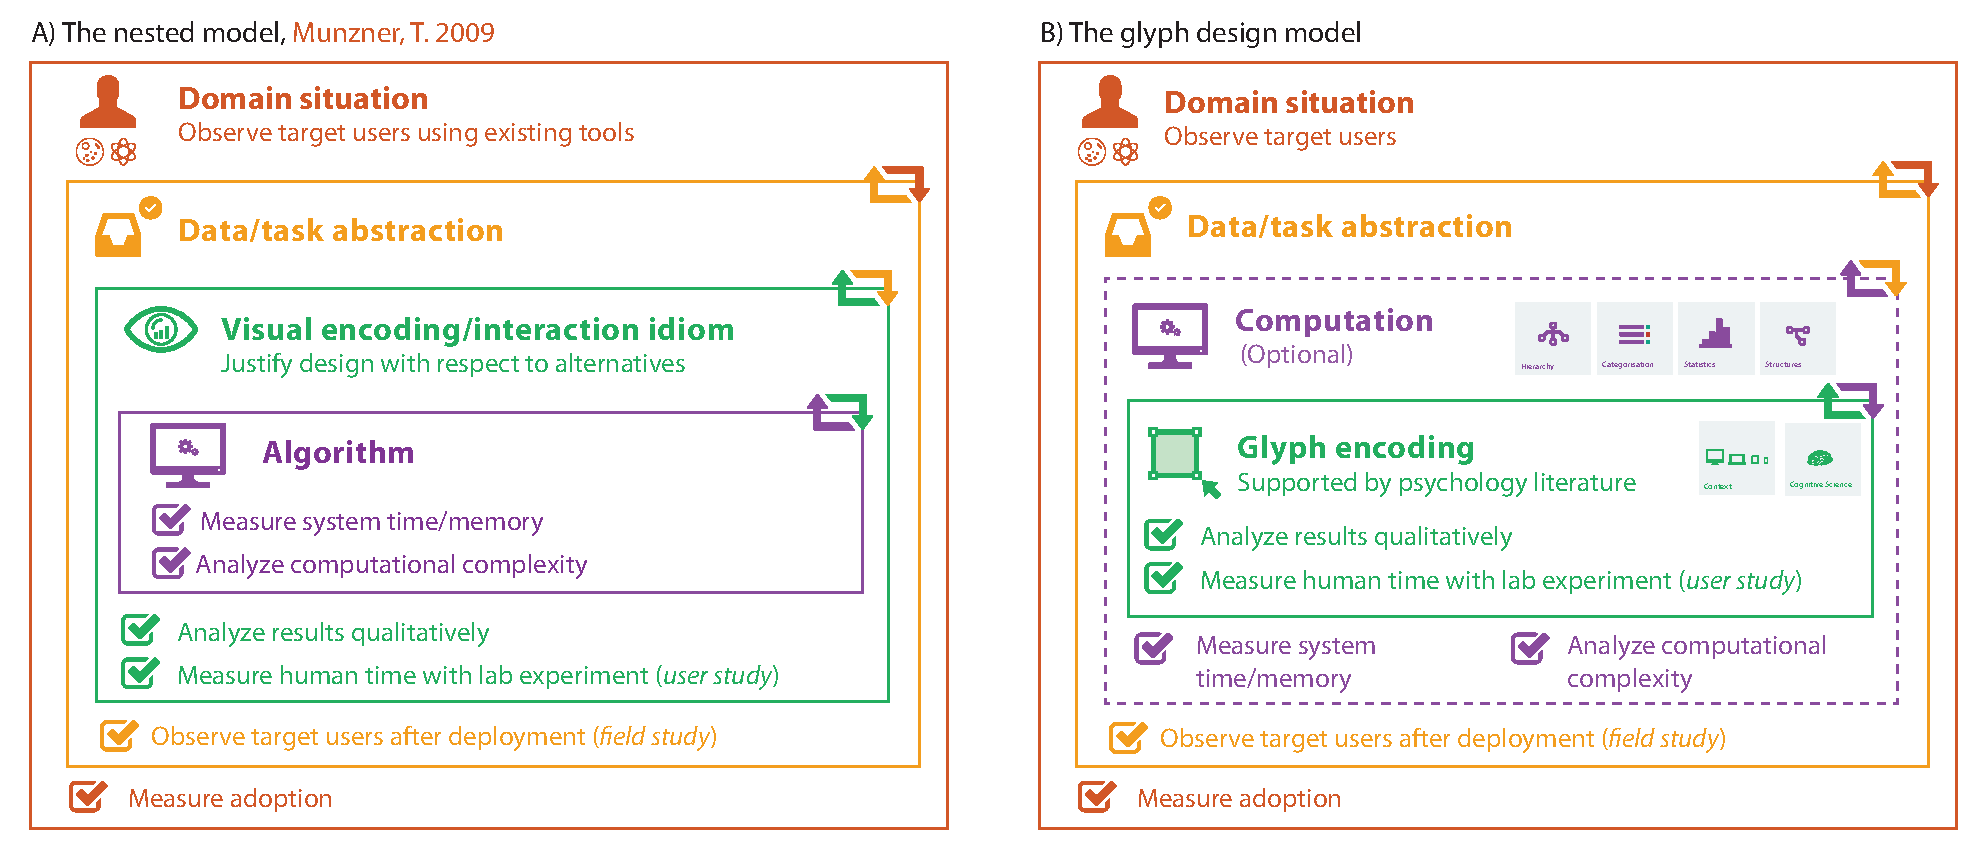
\includegraphics[width=\textwidth]{images/ch3/model}
%\caption{A) The ``nested model'' from Munzner \cite{munzner2009nested} provides a model for visualization design based on close interaction with domain experts and evaluation at each stage of the design process. The model supports an iterative design through feedback and feedforward loops between components.
%B). Our model integrates domain-expert interaction and evaluation along with design guidelines and computational techniques to create an overall model to support systematic glyph design. The computation element is optional since it is may not always be applicable.}
%\label{fig:model}
%\end{figure}
%
%Through integrating design guidelines and computational techniques with the ``nested model'' we can create a ``glyph design model'' shown in Figure \ref{fig:model} B.
%This model emphasizes the importance of domain-expert interaction and evaluation whilst placing computation in the middle to help in data/task abstraction as well as informing the visual encoding.
%
%\begin{figure}[h!]
%\centering
%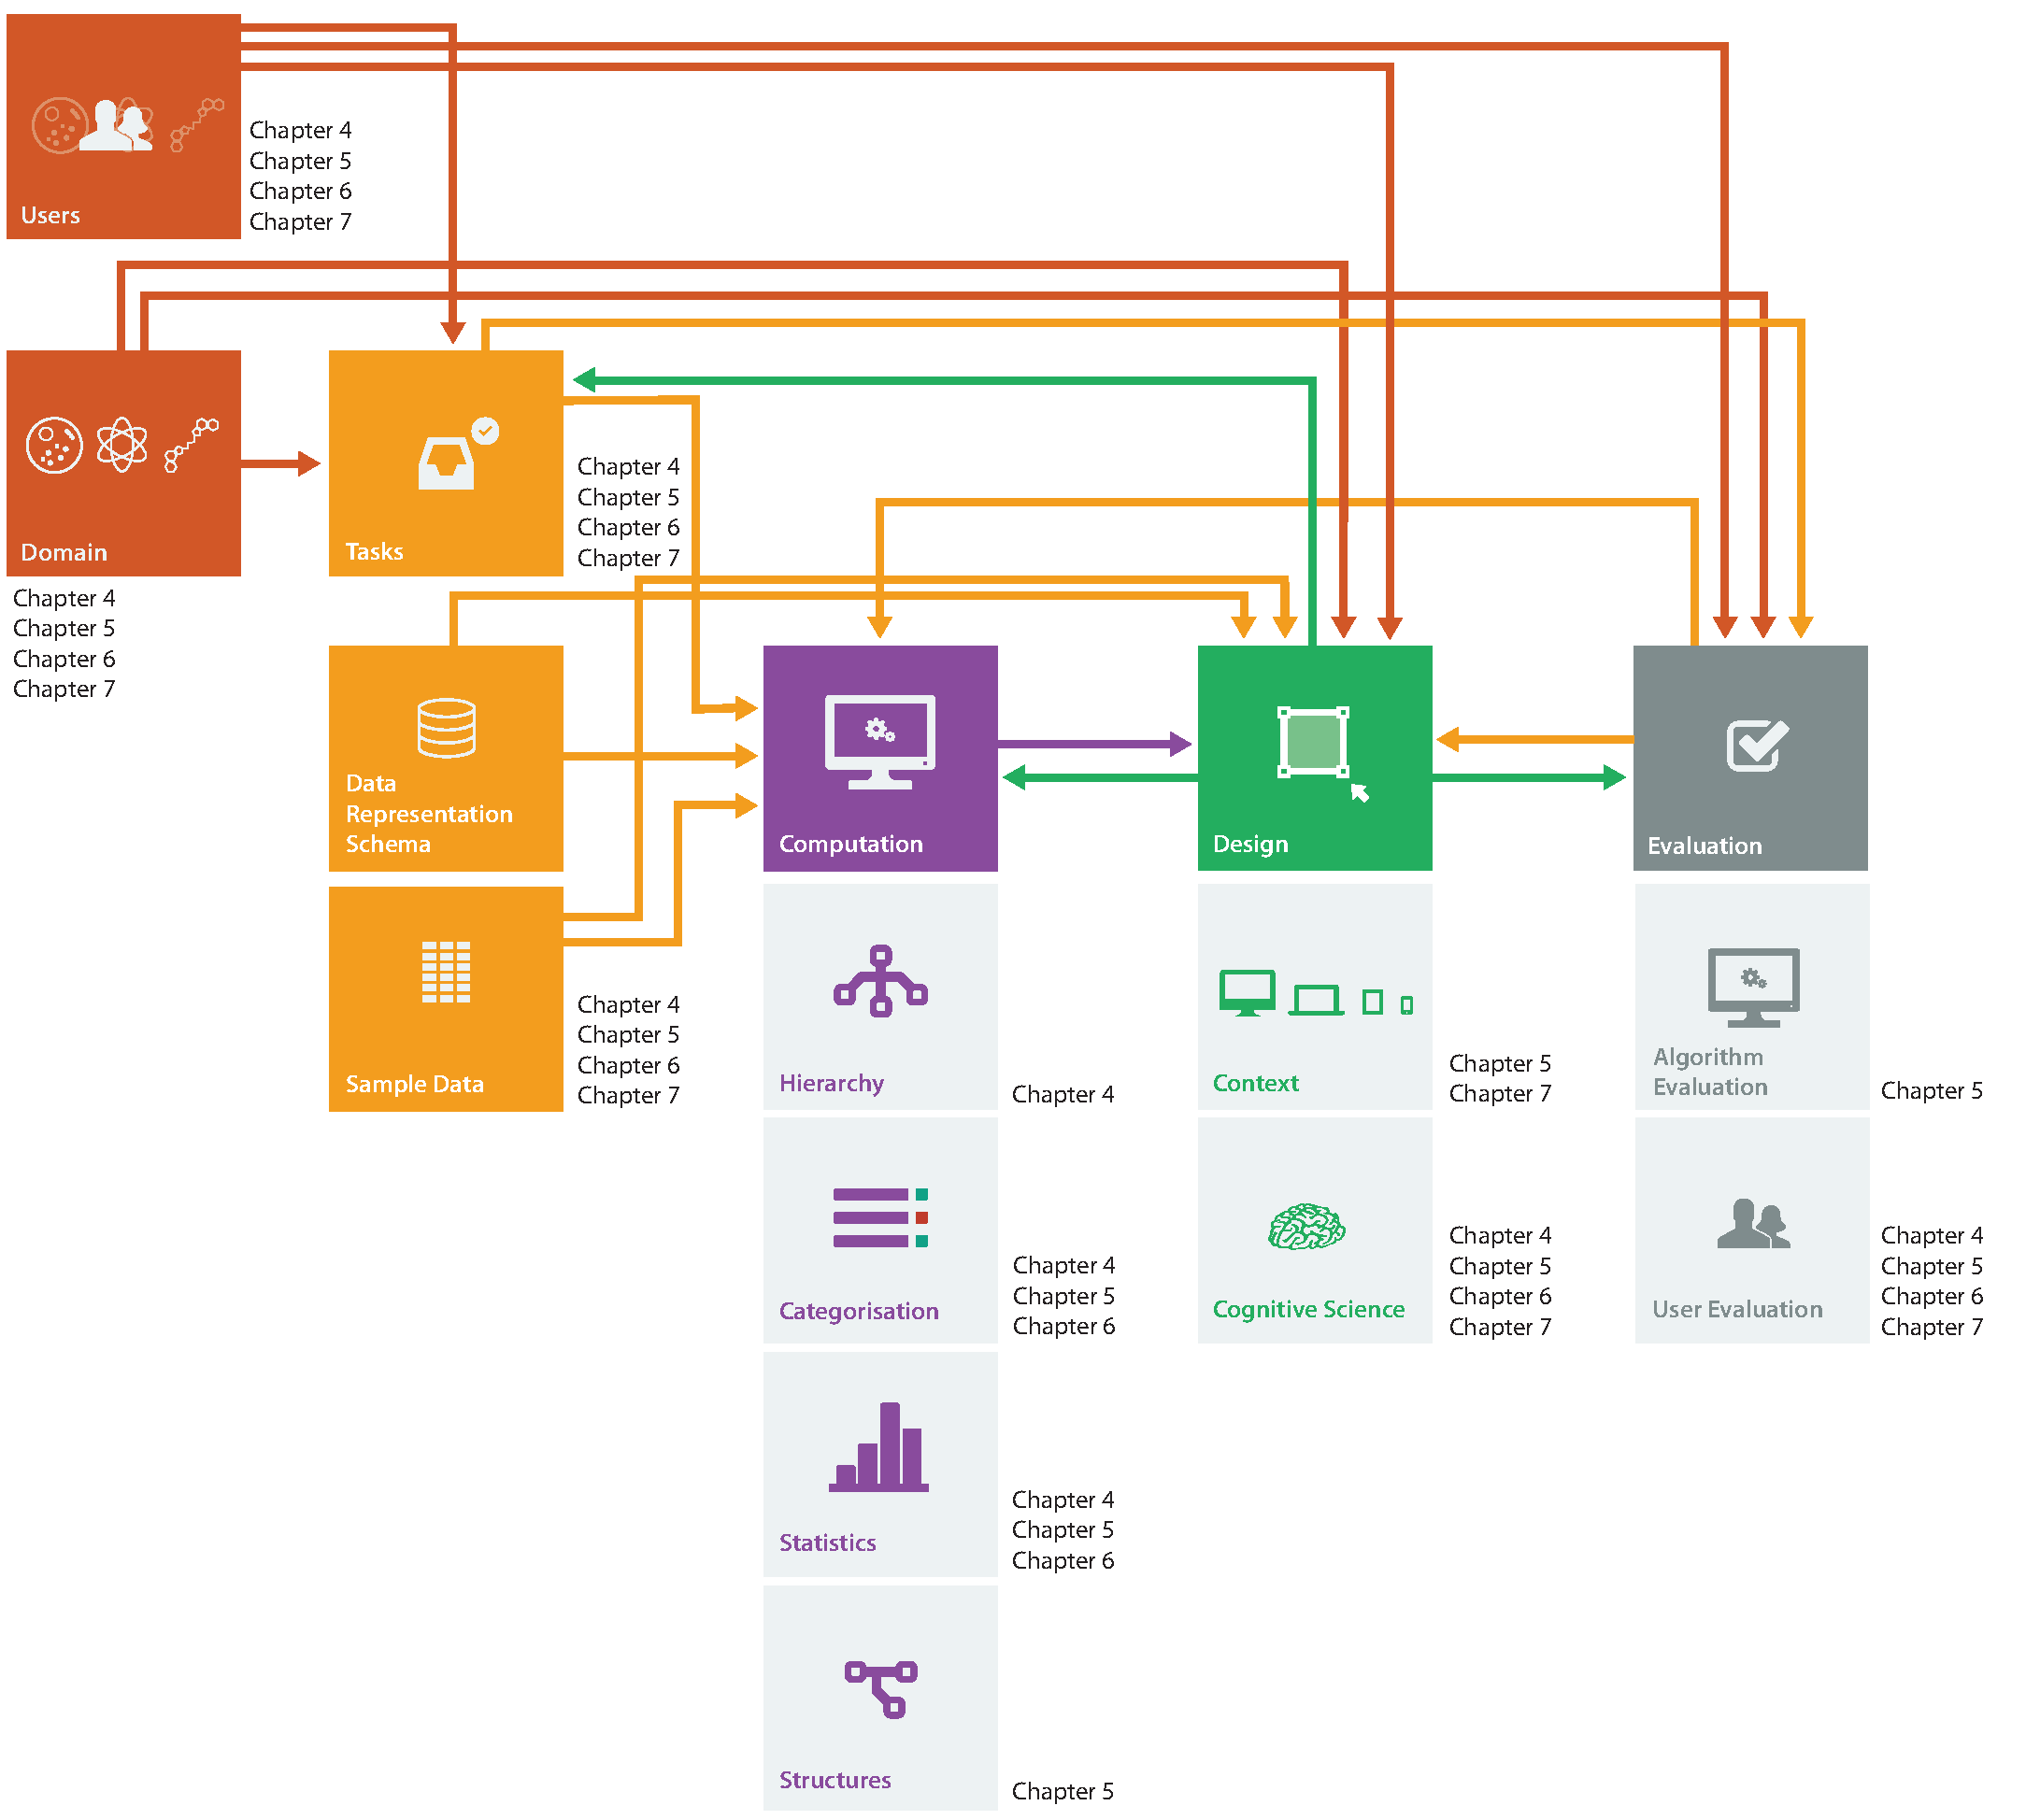
\includegraphics[width=\textwidth]{images/ch3/systematization}
%\caption{The model is formed by many interacting facets from initial requirements gathering through to the glyph design process. Marked on each process are the chapters that make use of that particular facet in the design process.}
%\label{fig:systematisation-process}
%\end{figure}
%
%Figure \ref{fig:systematisation-process} illustrates a more granular view of the model components and their dependencies, which are:
%
%\begin{itemize}
%\item \textbf{Users}, most often domain experts are the most important part of any design process, feeding in to:
%\begin{enumerate}
%	\item \emph{task} definition through interviews and day to day observations of current working practices;
%	\item \emph{design} processes via information about what a user is: willing to learn; willing to remember; and is able to remember. This ultimately affects the number of variables that can be encoded and how they are encoded. If a user has little time to remember glyphs, then they should be more accessible via increased use of metaphor for example; and 
%	\item \emph{evaluation} to determine whether or not the solution meets user expectations and solves the problem the glyph was meant for.
%\end{enumerate}
%\item \textbf{Domain} knowledge is of importance in any glyph design due to the importance of defining the tasks to be solved by the visualization properly. Furthermore domain knowledge carries further importance in glyph-based visualization due to the definition of metaphors to support learnability and memorability of the resulting glyphs;
%
%\item \textbf{Tasks} provide an indication of the types of visual queries that a user would like to make.
%These tasks form the basis of data prioritization.
%For example, if a major task performed by a user was finding users of a particular age, making the age information more visually available is important;
%
%\item \textbf{Data Representation Schema} - provides the available data types (\eg categorical or quantitative) that may be used to create a glyph. This in turn can be used in the design phase whereby guidelines from the psychology domain, presented in Chapter \ref{chap:related_work} can be applied to ensure that appropriate visual channels are used for particular data values;
%
%\item \textbf{Sample Data} gives an indication of the data values (and ranges) to be encoded by the glyphs. 
%These values can also be processed by algorithms to find the most common values, the rarest values, and so forth depending on the visualization requirements.
%
%\item \textbf{Computation} is a powerful way of processing the available data to determine a hierarchical organizations, categories, statistics, and structures in the data: 
%
%\item \textbf{Design} in addition to the design guidelines defined above, design can also be made better by consideration of:  
%	\begin{itemize}
%		\item \textbf{Context}, which defines the environment (\eg devices available) in which the glyphs are being used. \emph{Users} and their \emph{tasks} will have different requirements based on the environment being worked in.
%		If a set of glyphs are being presented on a power wall in a situation control room in one scenario versus a desktop in another, the glyphs may need to be designed differently. 
%		There would be little point in having thin lines with a high spatial frequency on a screen too far away for users to view. 
%		It would also be ill advised to use particular colours maps when 3D is a requirement since lighting effects such as shadowing can change how particular hues are rendered.
%		\item \textbf{Cognitive Science}:
%			\begin{itemize}
%				\item \emph{users} and their ability and/or willingness to learn and remember is an important consideration in any glyph design. 
%				A user with little time to learn a new visual language will not want very complex glyphs; and
%				For instance a cardiovascular surgeon using glyphs to show properties of the heart during surgery may not have the time to remember how five or six variables are mapped to retinal variable without having to consult a lookup chart;  
%				\item \emph{tasks} are important to cognitive science since variables that are important in achieving particular tasks can be emphasized more than variables of a lesser importance.
%				``High value'' information, important for completion of priority tasks should be visualized using powerful visual channels such as position or colour for example;
%				``Low value'' information that is more often utilized when diving in to more detailed views should be encoded using less powerful visual channels in less prominent positions within the glyph;
%				\item \emph{data schemas} provide an overview of the data types to be visualized including whether the values are quantitative or qualitative.
%				As shown in Chapter \ref{chap:related_work}, some visual channels are better suited to data type than others.
%				For example colour hue is not well suited to quantitative variables but position is. Conversely, colour hue works well as a means for representing categorical (qualitative) information;
%				\item \emph{data values} are useful at the design phase as a further way of determining a suitable mapping from the data value to its retinal variable.
%				For instance, for categorical information, it is estimated that between eight and twelve colours can be observed distinctly \cite{ware13}. If there are more categories it may be better to consider an alternative mapping; and
%				\item \emph{computational results} can provide the hierarchy, clusters, structures or statistics that may help in determining the most important features of the data. 
%				This in turn may be used to support the composition of the overall glyph.
%			\end{itemize}
%	\end{itemize}
%
%\item \textbf{Evaluation} provides some level of validation that the design that has been produced serves it purpose. 
%This can be validated by reviewing the tasks defined earlier with users to determine if the glyphs serve their purpose. 
%If glyphs are providing an alternative to an existing visualization system, benchmarks on user accuracy and task speed can be made for comparison purposes. 
%\end{itemize}
%
%These interlinked facets may be used in their entirety or selectively depending on the task.
%For instance, computation would not be required if the domain experts already knew the statistics, data hierarchy, structures or categories.
%In this case, that data can be directly fed in to the design stage.

\section{Summary}
We have set the scene and outlined a set of leads as to how glyph design could be made better, and described a ``model'' in Figure \ref{fig:new_process} to evaluate our idea.
The remainder of this thesis will apply this model to a number of scenarios and investigate how design guidelines and computation can contributed to the elaboration of a systematic glyph design process.

All further chapters will apply design guidance. They all however will differ in how computation is used (if at all), and in how evaluation is conducted.

\begin{enumerate}

\item \textbf{Chapter \ref{chap:glyph-tax}}:
\begin{itemize}
\item \emph{Users:} Biologists (domain experts involved in work).
\item \emph{Sample Data:} ArrayExpress \cite{ArrayExpress::2012} repository with over 1.2 million individual experiments.
\item \emph{Computation:} Categorization, statistical analysis, and hierarchical organization of biological sample characteristics (\eg, organism, organism parts) and processes.
\item \emph{Design:} Uses a computationally generated taxonomy in combination with retinal variable orderings and design guidelines.
\item \emph{Evaluation:} Domain expert evaluation.
\item \emph{Deployment:} Used in a popular data annotation and curation tool called ISAcreator \cite{rocca-serra10}.
\end{itemize}

\item \textbf{Chapter \ref{chap:automacron}}:
\begin{itemize}
\item \emph{Users:} Biologists (domain experts involved in work).
\item \emph{Sample Data:} ArrayExpress \cite{ArrayExpress::2012} repository with over 1.2 million biological experiments.
\item \emph{Computation:} Structure analysis of biological workflow graphs from Chapter \ref{chap:glyph-tax}, and statistical analysis.
\item \emph{Design:} Uses the motif finding algorithm to automatically generate multi-resolution glyphs by following design guidelines.
\item \emph{Evaluation:} Motif finding algorithm performance comparison and domain expert evaluation.
\item \emph{Deployment:} Available as a standalone tool for error detection tasks, and to build macro glyph libraries.
Also used in the ISAcreator \cite{rocca-serra10} tool to compress common patterns in biological workflows.
\end{itemize}

\item \textbf{Chapter \ref{chap:timeseries}}:
\begin{itemize}
\item \emph{Users:} General.
\item \emph{Sample Data:} Space shuttle and electrocardiogram data from Keogh \etal \cite{shuttle_data} .
\item \emph{Computation:} Statistical analysis to identify common time series patterns and count their occurrence.
\item \emph{Design:} Uses design guidelines to drive the glyph creation process.
\item \emph{Evaluation:} Baseline comparison with ground truth anomalies.
\item \emph{Deployment:} General purpose web application.
\end{itemize}

\item \textbf{Chapter \ref{chap:processes}} introduces a number of examples where computation does not always take centre stage.
These examples also use a more varied evaluation approach.
\begin{enumerate}
\item Biological sequence visualization:
\begin{itemize}
\item \emph{Users:} Biologists/Bioinformaticians.
\item \emph{Sample Data:} DNA sequences for the same region in 1809 bacteria.
\item \emph{Computation:} None.
\item \emph{Design:} Design guidelines followed to drive the glyph creation process.
\item \emph{Evaluation:} Domain expert involved in the design process throughout, followed by an online user survey with forty-two biologists and bioinformaticians.
\item \emph{Deployment:} Open-source sequence logo library viewer for the web.
\end{itemize}
\item Poetry visualization:
\begin{enumerate}
\item \emph{Poetry glyph}:
\begin{itemize}
\item \emph{Users:} Humanities scholars (poets).
\item \emph{Sample Data:} Numerous poetry, English texts and scientific literature.
\item \emph{Computation:} None.
\item \emph{Design:} Design guidelines followed to drive the glyph creation process.
\item \emph{Evaluation:} A number of poets and language scholars involved in the design process.
\item \emph{Deployment:} An online tool called PoemViewer \cite{CGF:Abd2013a}.
\end{itemize}
\item \emph{Macro glyph}:
\begin{itemize}
\item \emph{Users:} Humanities scholars (poets).
\item \emph{Sample Data:} Numerous poetry, English texts and scientific literature.
\item \emph{Computation:} Statistical and structural analysis.
\item \emph{Design:} Design guidelines followed to drive the glyph creation process.
\item \emph{Evaluation:} Semi-structured interviews.
\item \emph{Deployment:} An online tool called PoemViewer \cite{CGF:Abd2013a}.

\end{itemize}
\end{enumerate}

\item File system event visualization:
\begin{itemize}
\item \emph{Users:} General.
\item \emph{Sample Data:} Dropbox and Git log data.
\item \emph{Computation:} None.
\item \emph{Design:} Uses a new technique called the quasi-Hamming distance to create visually separable glyph designs that support error detection and correction.
\item \emph{Evaluation:} Computer- and user-based glyph similarity metrics for glyph designs.
\item \emph{Deployment:} Available in a file system visualization library called TreeLines.
\end{itemize}
\end{enumerate}


\end{enumerate}